
%\section*{Foreword}
%\begin{figure}[ht] 
%	
%	\centering
%	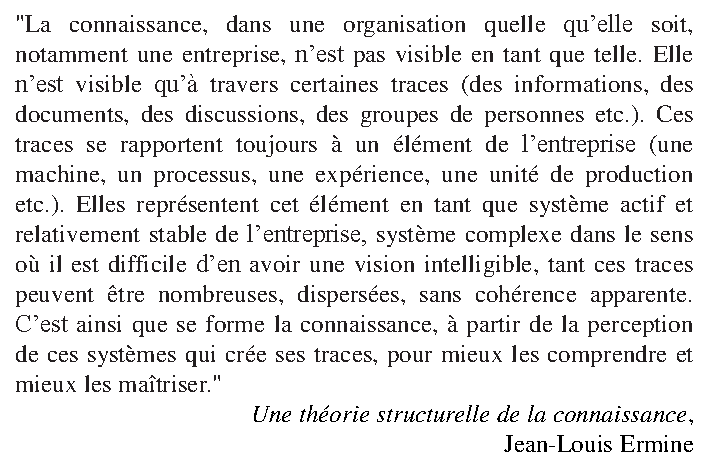
\includegraphics[width=.7\linewidth]{images/citation-ermine.pdf}
%\end{figure}



\section{Introduction}\label{sect:intro}
This document presents the integration of Trace\textit{a} \cite{batot2021-not-another-metamodel}, a language dedicated to traceability into the new release of SysML language.
It is the continuation of deliverables 1, 2, and 3 of the Trace\textit{a} project\footnote{Trace\textit{a} is part of the Modelia intiative which aims at "Bringing artificial intelligence to the modeling world"\\ \url{https://modelia.eu/projects/}.}. The first deliverable introduces the conceptualization work (SoA) related to traceability (D1)~\cite{deliverable1}. The second presents the metamodel of a language dedicated to traceability (D2) that fills the gaps detected in the existing literature during D1~\cite{deliverable2}. The third deliverable shows the evaluation and integration of functionalities (confidence and evidence) in a software dedicated to traceability (D3)~\cite{deliverable3}.
This report presents the integration of the concepts related to traceability developed during these first three deliverables within SysMLv2\footnote{We alternately use the names SysML and SysMLv2 to refer to SysMLv2. The distinction between the two as well as all documentation relating to KerML / SysMLv2 is available by following the link:\\ \url{https://github.com/Systems-Modeling}.}.

This document is organized as follows.
\Sect{sec:background}, first briefly introduces the language dedicated to traceability that we have developed as well as the KerML / SysMLv2 ecosystem on which we integrate it. This section also defines the high level needs for quality traceability.
\Sect{sec:strategies}, presents which elements of KerML / SysMLv2 languages are of interest and how we have adapted and used them through the different integration strategies considered.
We will detail our choices of architecture and implementation and the limits that we encountered in \Sect{sec:extension}\footnote{We are integrating Trace\textit{a} into SysMLv2 while it is being formalized by the SST.}.
Finally, we conclude this document in \Sect{sec:conclusion} before pointing at the resulting software artefacts and their examples of use in \Sect{sec:artefacts}.






% \begin{descriptioncompact}
%      \item[Suite de Tracea] Livrables, objectifs
     
%      \item[Besoins de SysML] Intérêt à intégré Tracea au nouveau standard 
%      - Limitations
%      - Niveau de priorité faible (retard de livraison)
     
%      \item[Stratégies explorées] Elements du noyau (cibles de la traçabilité)
%      \begin{itemize}
%          \item  \textbf{Approches naïves/intrusives:} Modifier les éléments du noyau - Nouveau type d'annotation)
%          \item \textbf{Approches orthogonales:} Nouvelle fonction annotatrice - Bibliothèque de fonctionnalités) 
%      \end{itemize}
% \end{descriptioncompact}


